

\fancypagestyle{miEstilo505}{
   \lhead{5.5 Interfaz de usuarion}
   \rhead{Página \thepage}
   \lfoot{}
   \cfoot{}
   \rfoot{}
}

\pagestyle{miEstilo505}

\subsection{Interfaz de usuario}

Para facilitar la interacción del usuario con la aplicación y mejorar su experiencia de usuario, se ha realizado un diseño de interfaz mediante botones e iconos (interfaz soportada por la API de telegram) utilizando los llamados 'Callback buttons` \cite{refx1}. Cuando un usuario pulsa estos botones, no se envía ningún mensaje al chat, sino que en su lugar el bot recibe una consulta que es manejada y respondida con una acción.

El diseño propuesto se basa en un modelo jerárquico, donde podremos ir realizando una navegación entre menús partiendo del menú principal.

Este diseño es el siguiente:

\textbf{AQUÍ VA EL DISEÑO DE LA INTERFAZ DE USUARIO} 

\newpage

Su implementación se basa en realizar un menú con un conjunto de botones con los que poder navegar. Por ejemplo, la siguiente figura muestra el menú principal, donde se puede acceder al conjunto de funcionalidades de la aplicación.

\begin{figure}[h]
	\centering
	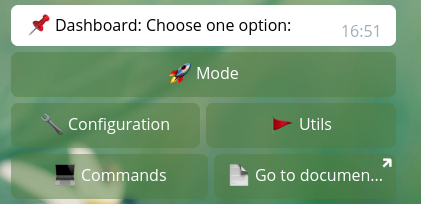
\includegraphics[scale=0.8]{images/42}
	\caption{Menú principal de la aplicación}
\end{figure}

En la sección de \textit{Mode} se podrá acceder al conjunto de acciones relacionados modos de uso de la aplicación, en \textit{Configuration} se podrá acceder al conjunto de opciones para configurar la cámara \ldots
Por ejemplo, si pulsamos el botón de \textit{Mode} se podrá acceder al conjunto de funcionalidades relacionadas.

\begin{figure}[h]
	\centering
	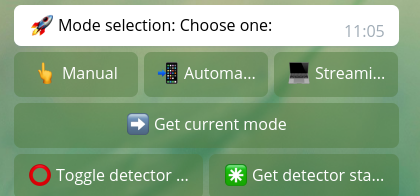
\includegraphics[scale=0.8]{images/39}
	\caption{Menú Mode}
\end{figure}

La implementación de esta interfaz se puede comprobar en este \href{https://github.com/jmv74211/TFM_security_system_PI/blob/master/src/agents/telegram_bot.py#L972}{enlace}.

\begin{tabular}{|p{15.5cm}|}
	
	\hline
	
	\textit{ \textbf{*Nota:} Para más información, todo este conjunto de botones y funcionalidades serán explicados en la guía de usuario de la sección X. }
	\\
	\hline
	
\end{tabular}

\newpage
